\documentclass{article}
\usepackage{graphicx} % Required for inserting images
\usepackage{physics}
\usepackage{mathrsfs}
\usepackage{amssymb}
\usepackage{graphicx}
\usepackage{color}
\title{NRG results and FRG results}
\begin{document}
\maketitle
\begin{figure}[!h]
    \centerline{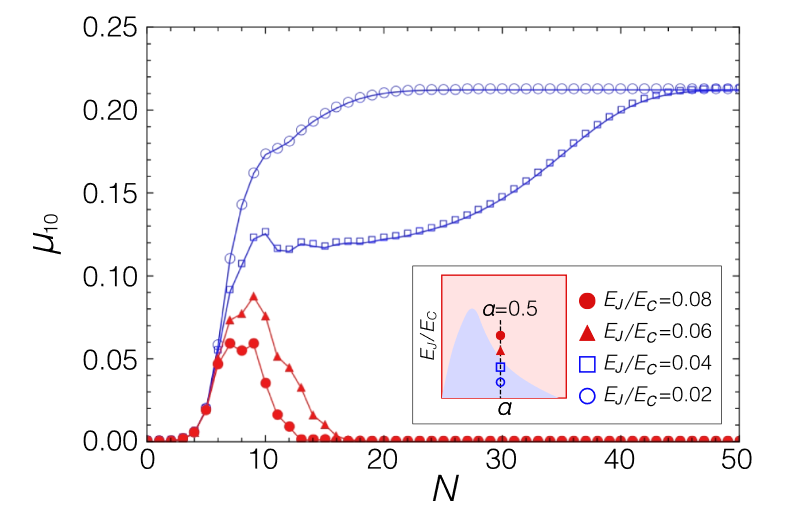
\includegraphics[width=\columnwidth]{Phy129087001_2.png}}
    \caption{Figure.3 Typical NRG Flows of $\mu_{10}$ at $\alpha=0.5$}
    \label{figure_3} 
\end{figure}

RG procedure : beginning :\\
\textcolor[rgb]{0,0,1.0}{ $\frac{E_J}{E_C} \leq 0.04 $ , $\mu_{10} \rightarrow$ grows, system : insulator phase.}\\
\textcolor{red}{$\frac{E_J}{E_C} \geq 0.04 $ (Threshold value) , $\mu_{10} \rightarrow$ decreases}\\
$\rightarrow$ determine critical values, method : extraplolting the wilson parameter. $\Lambda \rightarrow 1$ for each $\alpha$
\begin{figure}[!h]
    \centerline{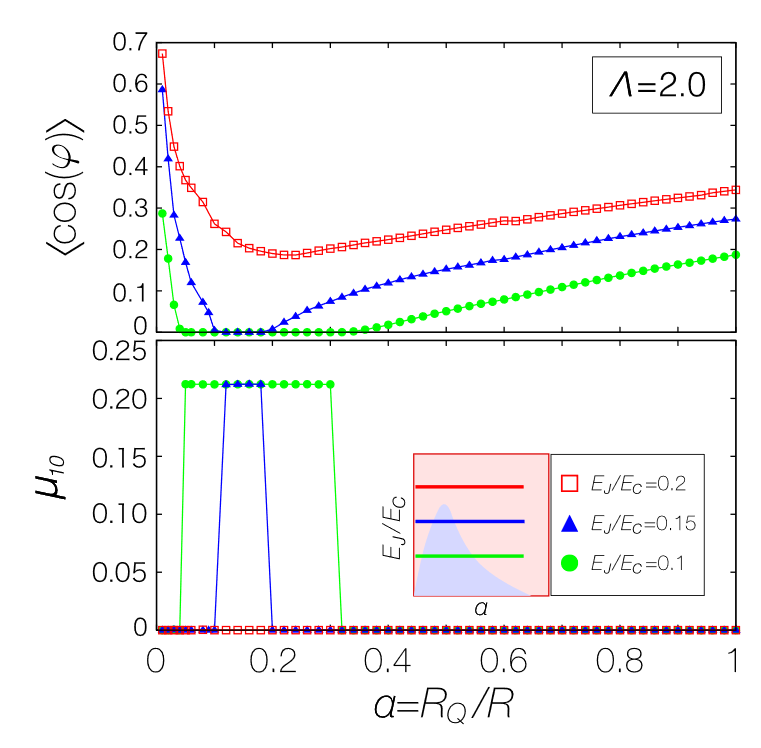
\includegraphics[width=\columnwidth]{Phy129087001_3.png}}
    \caption{Figure.4 $\langle \cos (\phi) \rangle$ (phase coherence), $\mu_{10}$ (mobility) at diff $\alpha$ and $\frac{E_J}{E_C}$.}
    \label{figure_4} 
\end{figure}
\\
 \\
\textcircled{1} behavior of $\langle \cos{\phi} \rangle$ and $\mu_{10}$ are \textbf{consist} with with other\\
\\
$\langle \cos{\phi} \rangle = 0$ , $\mu_{10} \neq 0$ : insulator phase (delocalized phase?)\\
$\langle \cos{\phi} \rangle \neq 0$ , $\mu_{10} = 0$ : superconductor phase (localized phase?)\\
\textcircled{2} $\langle \cos{\phi} \rangle$ and $\mu_{10}$ : indicate reentrant into SC phase\\
\\
NRG results on a deeper level $\rightarrow$ nonperturbative analytical approach, \textbf{Functional Renormalization Group}\\
$\langle $functional anstanz$\rangle$ : \\
\textcircled{1} most relevant Fourier model \\
\textcircled{2} $\cos (\phi)$  \\
\textcircled{3} local potential approx. \\
\\
flow equations : \\
 $d_J \ln \epsilon_J = 1- \int^{\infty}_{0}\frac{dy}{\pi}g(y)$\\
 $d_C \ln \epsilon^{-1}_C = -1 + \epsilon^{2}_J\int^{\infty}_{0}\frac{dy}{\pi}h(y)$
 \\
 \\
DQPT : Dissipative Quantum Phase transition \\
\\
presence of DQPT : at $\alpha_c$ =1\\
absence of DQPT : at $\alpha < 1 $
\end{document}